\section{Quy trình làm việc}

\subsection{Quy trình làm việc}
\hspace*{0.5cm} Nhóm thực hiện công việc với chu kì một tuần. Bắt đầu với công việc xem xét, xác định công việc cần làm trong tuần, lên kế hoạch và tiến hành thực hiện các công việc. Cuối mỗi chu kì, nhóm tiến hành họp báo cáo công việc đã hoàn thành, đồng thời bắt đầu chi kì tiếp theo, tiếp tục tính toán và lên kế hoạch cho công việc tuần tới.\\

Công việc chi tiết của mỗi tuần của nhóm được trình bày dưới đây:


{
\setlength\extrarowheight{6pt}
\begin{longtable}{| p{2cm} | p{2cm} | p{10cm} |}

    \hline
    \textbf{Bắt đầu} & \textbf{Hạn} & \textbf{Công việc}                                             \\
    \hline
    02/01/2023       & 08/01/2022   &
    - Phong: Setup môi trường cho CustomerUI và hiện thực layout.
    \newline
    - Hiển: Setup môi trường cho AdminUI và hiện thực layout.
    \newline
    - Thọ: Setup môi trường cho backend, khởi tạo các service và đảm bảo giao tiếp giữa các service. \\
    \hline
    09/01/2023       & 16/09/2022   &
    - Phong: Hiện thực Login page - Register page và Reset Password page.
    \newline
    - Hiển: Hiện thực Branch page - Branch detail page - Order page - Order detail page.
    \newline
    - Thọ: Hiện thực Customer service                                                                \\
    \hline
    30/01/2023       & 05/02/2022   &
    - Phong: Hiện thực Home page - List Product page.
    \newline
    - Hiển: Hiện thực Event page - Event detail page - Goods page - Goods detail page, Goods Edit page.
    \newline
    - Thọ: Hiện thực Cart service.                                                                   \\
    \hline
    06/02/2023       & 12/02/2022   &
    - Phong: Hiện thực Product Detail page - Cart page.
    \newline
    - Hiển: Hiện thực Staff page - Staff Detail page - Staff Request page.
    \newline
    - Thọ: Hiện thực Order service                                                                   \\
    \hline
    13/02/2023       & 19/02/2022   &
    - Phong: Hiện thực Payment page - Manager Order page.
    \newline
    - Hiển: Hiện thực Account page, Account Detail page.
    \newline
    - Thọ: Hiện thực Account service                                                                 \\
    \hline
    20/02/2023       & 26/02/2022   &
    - Phong: Hiện thực Order Detail page và Customer Info page.
    \newline
    - Hiển: Hiện thực Warehouse page - Statistic page.
    \newline
    - Thọ: Hiện thực Staff service.                                                                  \\
    \hline
    27/02/2023       & 05/03/2022   &
    - Phong: Refactor code cho CustomerUI, hiện thực Event service.
    \newline
    - Hiển: Refactor code cho AdminUI, hiện thực Statistic service.
    \newline
    - Thọ: Hiện thực Branch service.                                                                 \\
    \hline
    06/03/2023       & 12/03/2022   &
    - Hiển           \& Phong: Nghiên cứu, chuyển đổi BPMN sang BPEL
    \newline
    - Thọ: Hiện thực Warehouse service.                                                              \\
    \hline
    13/03/2023       & 19/03/2022   &
    - Hiển           \& Phong: Nghiên cứu, chuyển đổi BPMN sang BPEL
    \newline
    - Thọ: Hiện thực Goods service.                                                                  \\
    \hline
    20/03/2023       & 26/03/2022   &
    - Hiển           \& Phong: Nghiên cứu, chuyển đổi BPMN sang BPEL
    \newline
    - Thọ: Hiện thực Event service.                                                                  \\
    \hline
    27/03/2023       & 02/04/2022   &
    - Hiển           \& Phong: Nghiên cứu, chuyển đổi BPMN sang BPEL
    \newline
    - Thọ: Hiện thực Statistic service.
    \newline
    - Tất cả: Viết báo cáo                                                                           \\
    \hline
    03/04/2023       & 16/04/2022   &
    - Hiển           \& Phong: Nghiên cứu, chuyển đổi BPMN sang BPEL.
    \newline
    - Thọ: Hiện thực BFF và các adapter
    \newline
    - Tất cả: Viết báo cáo                                                                           \\
    \hline
    17/04/2023       & 23/04/2022   &
    - Hiển           \& Phong: Nghiên cứu, chuyển đổi BPMN sang BPEL.
    \newline
    - Thọ: Hiện thực kết nối Kafka
    \newline
    - Tất cả: Viết báo cáo                                                                           \\
    \hline
    24/04/2023       & 30/04/2022   &
    - Tất cả thành viên: Tổng hợp hệ thống.
    \newline
    - Tất cả: Viết báo cáo                                                                           \\
    \hline
    01/05/2023       & 07/05/2022   &
    - Hiển           \& Phong: Viết báo cáo và kiểm thử hệ thống
    \newline
    - Thọ: Triển khai hệ thống                                                                       \\
    \hline
    08/05/2023       & 14/05/2022   &
    - Tất cả thành viên: Viết báo cáo, kiểm thử hệ thống                                             \\
    \hline
    15/05/2023       & 29/05/2022   &
    - Tất cả thành viên: Chuẩn bị cho phản biện và bảo vệ đề tài                                     \\
    \hline
\end{longtable}

}

\newpage

\begin{figure}[h]
    \begin{center}
        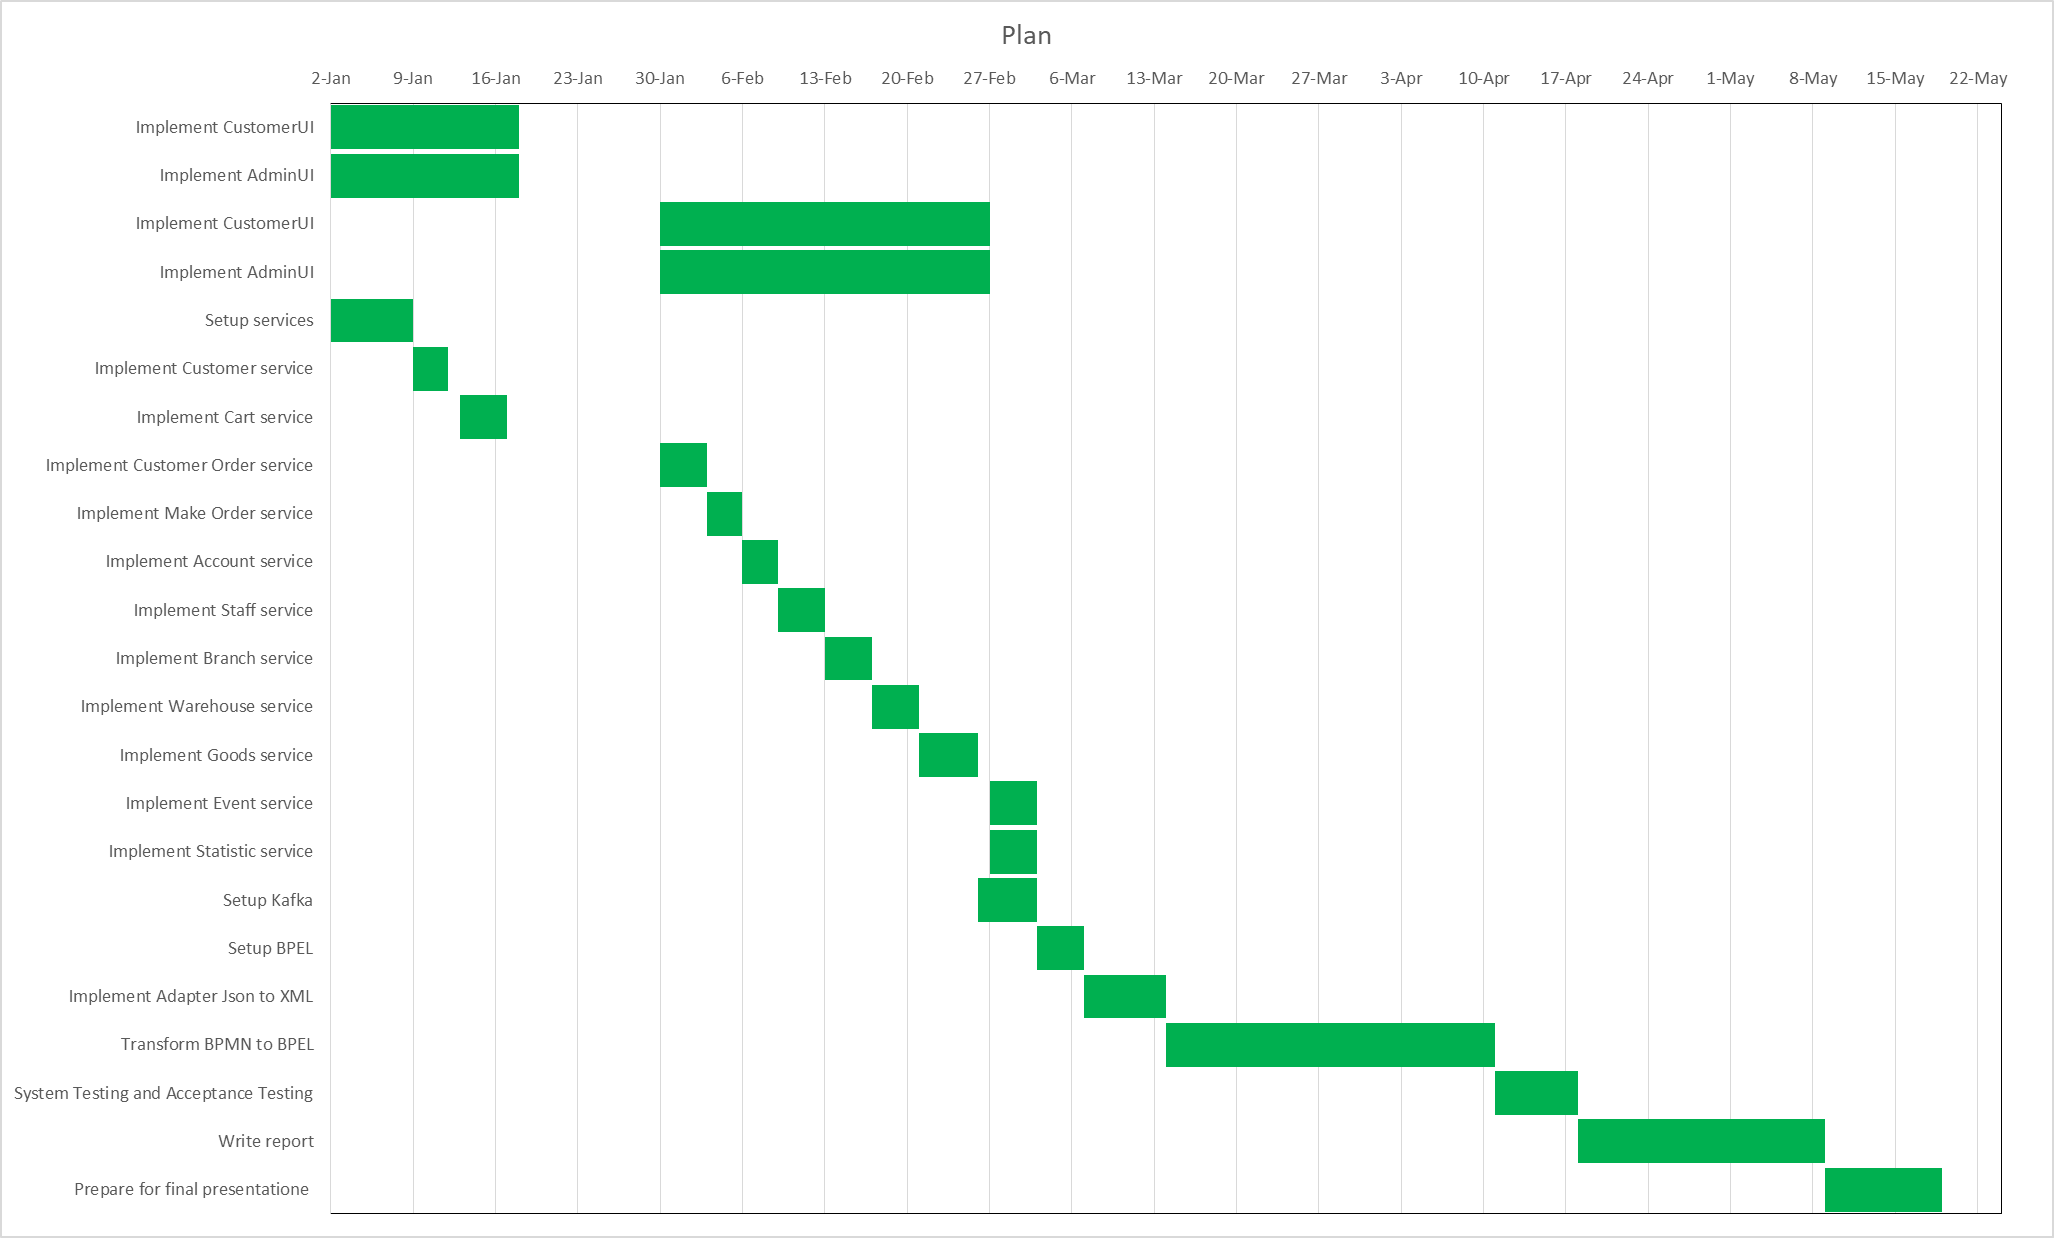
\includegraphics[width=14cm]{img/plan.png}
    \end{center}
    \caption{Biểu đồ Gantt quá trình thực hiện đồ án tốt nghiệp}
\end{figure}

\subsection{Quy trình phát triển phần mềm}
Nhóm đã phát triển hệ thông qua các quy trình sau:
\begin{itemize}
    \item Tìm hiểu nghiệp vụ của cửa hàng thời trang, đề xuất ra các chức năng cho hệ thống.
    \item Tiến hành thiết kế hệ thống bao gồm usecase, quy trình nghệp vụ, kiến trúc hệ thống, cơ sở dữ liệu và các giao diện.
    \item Hiện thực xây dựng hệ thống với việc xây dựng front-end, back-end và BPEL.
    \item Thực hiện kiểm thử hệ thống ở các mức đơn vị, mức tích hợp và mức hệ thống.
    \item Thực hiện triển khai hệ thống lên nền tảng đám mây.
\end{itemize}

\subsection{Phân chia công việc}
Tổng kết công việc của các thành viên như sau:

{
\setlength\extrarowheight{6pt}
\begin{longtable}{| p{4.5cm} | p{8cm} | p{2.5cm} |}

    \hline
    \textbf{Thành viên} & \textbf{Công việc}                                                                                         & \textbf{Hoàn thành} \\
    \hline
    %%%%%%%%%%%%%%%%%%%%%%
    Bùi Lương Vinh Hiển & - Hiện thực giao diện quản trị viên
    \newline
    - Hiện thực Event Service, Cart Service
    \newline
    - Thực hiện chuyển đổi BPMN và xây dựng quy trình BPEL
    \newline
    - Viết báo cáo      &
    100\%                                                                                                                                                  \\
    \hline
    %%%%%%%%%%%%%%%%%%%%%%
    Trần Tuấn Phong     & - Hiện thực giao diện khách hàng
    \newline
    - Thực hiện chuyển đổi BPMN và xây dựng quy trình BPEL
    \newline
    - Viết báo cáo      &
    100\%                                                                                                                                                  \\
    \hline
    %%%%%%%%%%%%%%%%%%%%%%
    Trần Nguyễn Hữu Thọ & - Hiện thực Branch Service, Staff Service, Account Service, Goods Service,Warehouse Service, Order Service
    \newline
    - Hiện thực BFF
    \newline
    - Triển khai hệ thống
    \newline
    - Viết báo cáo      &
    100\%                                                                                                                                                  \\
    \hline
\end{longtable}

}